%%%%%%%%%%%%%%%%%%%%%%%%%%%%%%%%%%%%%%%%%%%%%%%%%%%%%%%%%%%%%%%%%%%%%
%% Copyright (c) 2021- by Otacilio 'Minho' Neto, <minhotmog@gmail.com>
% This code is licensed under GPL 3 (see <https://www.gnu.org/licenses/> )
%%%%%%%%%%%%%%%%%%%%%%%%%%%%%%%%%%%%%%%%%%%%%%%%%%%%%%%%%%%%%%%%%%%%%
\documentclass[8pt,aspectratio=169]{beamer}
\usetheme[hidesidebar]{Corgi}
\setbeamercovered{transparent}	% Makes <onslide> elements translucid

%%%%%%%%%%%%%%%%%%%%%%%%%%%%%%%%%%%%%%%%%%%%%%%%%%%%%%%%%%%%%%%%%%%%%
%% This file is part of Minho's Corgi Beamer Theme.
%% Copyright (c) 2021-- by Otacilio 'Minho' Neto, <otacilio.neto@aalto.fi>
%
% This program is free software: you can redistribute it and/or modify
% it under the terms of the GNU General Public License as published by
% the Free Software Foundation, either version 3 of the License, or
% (at your option) any later version.
%
% This program is distributed in the hope that it will be useful, but
% WITHOUT ANY WARRANTY; without even the implied warranty of MERCHANTABILITY
% or FITNESS FOR A PARTICULAR PURPOSE. See the GNU General Public License
% <https://www.gnu.org/licenses/> for more details.
%
% The above copyright notice and this permission notice shall be included 
% in all copies or substantial portions of the Software.
%
%%%%%%%%%%%%%%%%%%%%%%%%%%%%%%%%%%%%%%%%%%%%%%%%%%%%%%%%%%%%%%%%%%%%%

% --------------------------------------------------------------------
% Packages
% --------------------------------------------------------------------
% Text, input, language-related packages
\usepackage[utf8]{inputenc}
\usepackage[T1]{fontenc}
\usepackage[english]{babel}
\usepackage[protrusion=true,expansion=true]{microtype} 
\usepackage{lmodern}

% Math packages
\usepackage{amsmath,amsfonts,amsthm,amssymb,bm,mathtools}

% Graphic and color packages
\usepackage[skins]{tcolorbox}				% Coloured boxes for LaTeX objects
\usepackage{graphicx} 						% Enhanced support for graphics
\usepackage{color, xcolor}					% Driver-independent color extensions

% General utilities
\usepackage[nodayofweek]{datetime}			% Customize date commands
\usepackage[document]{ragged2e}				% Text-alignment (\centering, ...)
\usepackage[ruled,vlined]{algorithm2e}		% Pseudo-code environment
\usepackage{algorithmic}					% Pseudo-code environments (beamer-friendly)
\usepackage{framed, mdframed}				% Framed and shaded environments
\usepackage{enumitem}						% Functionalities for {enumerate/itemize}
\usepackage{environ}						% Better interface for environments
\usepackage{listings}						% Coding environments
\usepackage{etoolbox,xstring}				% Environment hooks (\BeforeBegin...)
\usepackage{fontawesome}					% Font-awesome web icons
\usepackage{booktabs}						% Better {tabular} environments

% --------------------------------------------------------------------
% Packages Configurations
% --------------------------------------------------------------------
% (inputenc, fontenc): Set serif on math fonts
\usefonttheme[onlymath]{serif} 
\renewcommand{\familydefault}{\rmdefault}

% (minted): Set Monokai as default color style
%\usemintedstyle{monokai}
\definecolor{bg}{HTML}{282828} % (Source: https://github.com/kevinsawicki/monokai) 

% (enumitem): Default configurations for all lists
\setlist[itemize,1]{label=$\blacktriangleright$, format=\color{monokaiOrange}}
\setlist[itemize,2]{label=$\leadsto$, format=\color{monokaiOrange}}

% (listings): Defines the code styling and formatting
\lstset{
    backgroundcolor=\color[RGB]{39,40,34},
    language=matlab, keywordstyle=\color[RGB]{102,217,239},
    basicstyle=\footnotesize \ttfamily,breaklines=true,
    escapeinside={\%*}{*)}
}

% (datetime): Personalized date commands (apply them before a \today)
\newdateformat{datenum}{\twodigit{\THEDAY}/\twodigit{\THEMONTH}/\THEYEAR}
\newdateformat{datefull}{\twodigit{\THEDAY}{ }\monthname[\THEMONTH], \THEYEAR}

% (algorithm2e): Remove algorithm numbering
\renewcommand{\thealgocf}{}

% --------------------------------------------------------------------
% Commands
% --------------------------------------------------------------------

% Single line {itemize} environment
\newcommand{\pointer}[2]{%
	\IfEqCase{#1}{%
		{1}{\begin{itemize} \item #2 \end{itemize}}%
		{2}{\begin{itemize} \item[$\leadsto$] #2 \end{itemize}}%
	}[\PackageError{pointer}{Undefined option to pointer: #1}{}]%
}

% Clear separator line 
\newcommand{\separatorLine}[2]{\vskip#1{\color{monokaiBG!10!white}\hrule}\vskip#2}

% Fast colouring commands
\newcommand{\clP}[1]{{\color{monokaiOrange!66!black} #1}}
\newcommand{\clX}[1]{{\color{stateColor} #1}}
\newcommand{\clU}[1]{{\color{inputColor} #1}}
\newcommand{\clY}[1]{{\color{outputColor} #1}}
\newcommand{\clW}[1]{{\color{disturbanceColor} #1}}

\newcommand{\clPX}[1]{{\color{outputColor!75!black} #1}}
\newcommand{\clPU}[1]{{\color{inputColor!75!black} #1}}

% Colored hyperlinks
\newcommand{\chref}[2]{
  \href{#1}{{\usebeamercolor[bg]{Feather}#2}}
}

% A cooler transpose symbol 'T'
\newcommand*{\tran}{{\mkern-1.5mu\mathsf{T}}}

% Argmax and Argmin math operators
\DeclareMathOperator*{\argmax}{arg\,max}
\DeclareMathOperator*{\argmin}{arg\,min}

% Adds transparency to figures in overlays
\newcommand<>{\uncovergraphics}[2][{}]{
    % Taken from: <https://tex.stackexchange.com/a/354033/95423>
    \begin{tikzpicture}
    \node[anchor=south west,inner sep=0] (B) at (4,0) 
		{\includegraphics[#1]{#2}};
    \alt#3{}{%
        \fill [draw=none, fill=white, fill opacity=0.9] (B.north west) -- (B.north east) -- (B.south east) -- (B.south west) -- (B.north west) -- cycle;
    }
    \end{tikzpicture}
}

% Info and warning coloured boxes
\newcommand{\boxHighlight}[2][\textwidth]{
	\begin{center} 
	\begin{tcolorbox}[width=#1, boxsep=-2pt, frame empty, colback=monokaiBG!10!white, rounded corners]
		\faFileTextO~~#2
	\end{tcolorbox}
	\end{center}
}

\newcommand{\boxInfo}[2][\textwidth]{
	\begin{center} 
	\begin{tcolorbox}[width=#1, boxsep=-2pt, frame empty, colback=aaltoBlue!10!white, rounded corners]
		\color{aaltoBlue!80!white}
		\faInfoCircle~~#2
	\end{tcolorbox}
	\end{center}
}

\newcommand{\boxWarning}[2][\textwidth]{
	\begin{center} 
	\begin{tcolorbox}[width=#1, boxsep=-2pt, frame empty, colback=aaltoRed!10!white, rounded corners]
		\color{aaltoRed!80!white}
		\faWarning~~#2
	\end{tcolorbox}
	\end{center}
}

% --------------------------------------------------------------------
% Environments
% --------------------------------------------------------------------

% A shaded-block of variable size
\newenvironment<>{varblock}[2][.9\textwidth]
	{%
	\begin{minipage}[t]{#1}\centering%
	\begin{actionenv}#3%
		\def\insertblocktitle{#2}%
		\par%
		\usebeamertemplate{block begin}
	}
	{
		\par%
		\usebeamertemplate{block end}%
	\end{actionenv}
	\end{minipage}
	}
	% Includes beamer-specific preamble configurations

% FRONT MATTER ----------------------------------------------------------------
\title[Predictive control and equilibrium-seeking for WRRFs]{Predictive control and feedback equilibrium\\seeking for sustainable water resource recovery}
\subtitle[]{}
\author[O. Neto]{      
	Otacílio ``Minho'' Neto \\[2ex]
	{\footnotesize Process Systems Engineering (CMET/CHEM),\\[-1ex]Aalto University, Finland}
}

\institute[PSE-Seminars, 09.2025]{
	{\bfseries {Seminars on Process Systems Engineering}}\\
	Aalto University, September 25, 2025\\
  
	% /\ Compulsory empty line
}

% DOCUMENT --------------------------------------------------------------------
\begin{document}

% TITLE PAGE ------------------------------------------------------------------
{\1 
\begin{frame}[plain,noframenumbering] 
	\titlepage
\end{frame}
} 

% SLIDES ----------------------------------------------------------------------
% -----------------------------------------------------------------------------
\section{Introduction}
% -----------------------------------------------------------------------------
\begin{frame}[c]
\frametitle{Predictive control, operating WWTPs as self-sufficient WRRFs} \justifying

\boxHighlight[0.95\textwidth]{ \centering
    \textbf{Paradigm shift:} Wastewater as a sustainable source of water, energy, and raw materials
}

\vfill

\begin{center}
    \hspace*{-18em}\includegraphics<1>[width=1.15\textwidth]{figs/ControlFramework_01}%
\end{center}

\vfill

\end{frame}

% -----------------------------------------------------------------------------
\section{(Proposal A)\\Predictive control for transitioning WWTPs\\ into self-sufficient WRRFs} \sectioncover
% -----------------------------------------------------------------------------
\begin{frame}[c]
\frametitle{Predictive control, operating WWTPs as self-sufficient WRRFs} \justifying

\vskip1em

\boxHighlight[0.9\textwidth]{ \centering
    We consider the task of operating a \textbf{biological wastewater treatment plant} (WWTP, secondary treatment) as a \textbf{water resource recovery facility} (WRRF)
}

\vfill

\begin{center}
    \includegraphics<1>[width=\textwidth]{figs/ControlFramework_01}%
    \includegraphics<2>[width=\textwidth]{figs/ControlFramework_02}%
\end{center}

\vfill

\end{frame}

%------------------------------------------------------- 
\begin{frame}[t]
\frametitle{Predictive control, general architecture and specific configuration}\justifying

\vskip0.66em

\begin{columns}
	\column[t]{0.5\textwidth}
	\begin{center}
		\vskip-1.5em
		\includegraphics<1>[width=0.98\columnwidth]{figs/Control_Diagram_Isolated}% 
		\includegraphics<2>[width=0.98\columnwidth]{figs/Control_Diagram_Isolated_H1}% 
		\includegraphics<3>[width=0.98\columnwidth]{figs/Control_Diagram_Isolated_H3}% 
		\includegraphics<4>[width=0.98\columnwidth]{figs/Control_Diagram_Isolated_H2}% 
	\end{center}

	\column[t]{0.49\textwidth}
	We design a \textbf{model-based} output-feedback controller
    \begin{equation*}
        \Sigma \coloneqq \left\{
            \begin{aligned}
                \textstyle\frac{d}{dt}\clX{x(t)} &= f(\clX{x(t)}, \clW{w(t)}, \clU{u(t)})   & \text{\footnotesize\color{gray}(dynamics)} \\
                \clY{y(t)}   				     &= g(\clX{x(t)}, \clW{w(t)}, \clU{u(t)})   & \text{\footnotesize\color{gray}(measurements)} \\
                \clY{z(t)}   				     &= h(\clX{x(t)}, \clW{w(t)}, \clU{u(t)})   & \text{\footnotesize\color{gray}(performance)}
            \end{aligned}
        \right.
    \end{equation*}

	\vskip0.5em
	which autonomously operates the plant in cycles	
	\begin{center}
		\includegraphics[width=0.9\columnwidth]{figs/Control_Diagram_Time}
	\end{center}
\end{columns}

\vskip2em

\only<2>{\centering%
    \begin{tcolorbox}[colframe=monokaiBG!33!white, colback=white, width=\textwidth, rounded corners]
    \vspace*{-1.66em}
    \begin{tcolorbox}[frame empty, boxsep=-5pt, colback=white, width=19em]
        \textsc{Operating point optimizer} | $\mathrm{OPO}(\cdot)$
    \end{tcolorbox} 
    \vspace*{-0.33em}
    \begin{columns}
    \column[c]{0.45\columnwidth}
    \vskip-2em
    \begin{align*}
        \underset{x_k,~ u_k}{\text{minimize}} \quad
        & \left\| 
                \clP{\begin{bmatrix} W_{z|\text{ref}} & \\ & W_{u|\text{ref}} \end{bmatrix} }
                \begin{bmatrix} 
                    \clY{z_k - \bar{z}^{\text{ref}}_k} \\ 
                    \clU{u_k - \bar{u}^{\text{ref}}_k} 
                \end{bmatrix} 
        \right\|_2^2 \\
        \underset{}{\text{subject to}} \quad
            &  0  = f(\clX{x_k}, \clW{\bar{w}^{\text{ref}}_k}, \clU{u_k}) \\[-2ex]
            % & z_k = h(x_k, \bar{w}^{\text{ref}}_k, u_k) \label{eq: WRRF_OPO_c}\\
            & \clY{z_k \in \mathcal{Z}_{\text{ref}}}, ~~ \clX{x_k \in \mathcal{X}_{\text{ref}}}, ~~ \clU{u_k \in \mathcal{U}_{\text{ref}}}
    \end{align*}

    \column[c]{0.1em}\rule{0.5pt}{6em}

    \column[c]{0.54\columnwidth} 
    \vskip-2em
    \begin{equation*}
        \hspace*{-1em}
        \Sigma^{\delta|k} \coloneqq \left\{
        \begin{aligned}
            \clP{z}\clX{x^{\delta}[n]} &= \clP{A_k} \clX{x^{\delta}[n]} + \clP{B_{w|k}} \clW{w^{\delta}[n]} + \clP{B_{u|k}} \clU{u^{\delta}[n]} \\
                           \clY{y^{\delta}[n]} &= \clP{C_k} \clX{x^{\delta}[n]} + \clP{D_{w|k}} \clW{w^{\delta}[n]}
        \end{aligned}
        \right.
    \end{equation*}
    \end{columns}
    \end{tcolorbox}
}%
\only<3>{\centering%
    \begin{tcolorbox}[colframe=monokaiBG!33!white, colback=white, width=\textwidth, rounded corners]
        \vspace*{-1.66em}
        \begin{tcolorbox}[frame empty, boxsep=-5pt, colback=white, width=20.5em]
            \textsc{Model predictive controller} | $\mathrm{MPC}(\cdot)$
        \end{tcolorbox} 
        \vspace*{-2em}
        \begin{align*}
            \underset{\clU{u^{\delta}[\cdot]},~ \clX{x^{\delta}[\cdot]}}{\text{minimize}} \quad
            & \sum_{n=0}^{N_c-1} \left\| 
                    \clP{\begin{bmatrix} W_{x|n} & \\ & W_{u|n} \end{bmatrix}} 
                    \begin{bmatrix} 
                        \clX{x^{\delta}[n]}  \\ 
                        \clU{u^{\delta}[n]}
                    \end{bmatrix} 
            \right\|_2^2 + \left\| \clP{W_{x|N_c}} \clX{x^{\delta}[N_c]} \right\|_2^2 \\
            \underset{}{\text{subject to}} \quad
                &  \Sigma^{\delta|k} \text{ with } \clW{w^{\delta}[n] = \hat{w}^{\delta}_{N_e{-}1}} \text{ and } \clX{x^{\delta}[0] = \hat{x}^{\delta}_{N_e}} \\[-1.5ex]
                &  \clX{x^{\delta}_{\text{lb}} \preceq x^{\delta}[n] \preceq x^{\delta}_{\text{ub}}}, 
                ~~ \clU{u^{\delta}_{\text{lb}} \preceq u^{\delta}[n] \preceq u^{\delta}_{\text{ub}}}
        \end{align*}
    \end{tcolorbox}
}%
\only<4>{\centering
    \begin{tcolorbox}[colframe=monokaiBG!33!white, colback=white, width=\textwidth, rounded corners]
        \vspace*{-1.66em}
        \begin{tcolorbox}[frame empty, boxsep=-5pt, colback=white, width=19em]
            \textsc{Moving horizon estimator} | $\mathrm{MHE}(\cdot)$
        \end{tcolorbox} 
        \vspace*{-2em}
        \begin{align*}
            \underset{\clW{w^{\delta}[\cdot]},~ \clX{x^{\delta}[\cdot]}}{\text{minimize}} ~~
            & \sum_{n=0}^{N_e-1} \left\| 
                    \clP{\begin{bmatrix} W_{y|n} \hspace*{2.6em} \\ \hspace*{2.6em} W_{w|n} \end{bmatrix}} \hspace*{-0.25em}
                    \begin{bmatrix} 
                        \clY{y^{\delta}[n] {-} y^{\text{data}|\delta}_n}  \\ 
                        \clW{w^{\delta}[n] {-} w^{\text{data}|\delta}_n}  
                    \end{bmatrix} 
            \right\|_2^2 {+} \left\| \clP{W_{y|N_e}} \clY{\big( y^{\delta}[N_e] {-} y^{\text{data}|\delta}_{N_e} \big)} \right\|_2^2 \\
            \underset{}{\text{subject to}} ~~
                &~ \Sigma^{\delta|k} \text{ with } \clU{u^{\delta}[n] = u^{\text{data}|\delta}_n}\\[-1.5ex]
                &~ \clX{x^{\delta}_{\text{lb}} \preceq x^{\delta}[n] \preceq x^{\delta}_{\text{ub}}}, 
                ~~ \clW{w^{\delta}_{\text{lb}} \preceq w^{\delta}[n] \preceq w^{\delta}_{\text{ub}}}. 
        \end{align*}
    \end{tcolorbox}
}%

\end{frame}

% -----------------------------------------------------------------------------
\begin{frame}[t]
\frametitle{Predictive control, experimental study}\justifying
	
\vskip1em

\boxHighlight[0.9\textwidth]{ \centering
    We consider the task of operating a \textbf{biological wastewater treatment plant} (WWTP, secondary treatment) as a \textbf{water resource recovery facility} (WRRF)
}

\vfill

\begin{columns}
	\column[c]{0.45\textwidth}%
	\includegraphics[width=\columnwidth]{figs/WRRF_Schematic_Instrumented_Colors}

	\column[c]{0.54\textwidth}
	\begin{itemize}
		\item {\color{monokaiOrange}\sc Primary objective:}\\
		on demand, produce effluent water of specific quality
		\vskip0.5em
		\begin{center}
            \begin{tabular}{@{}c ccc@{}} \toprule
                Water class & \multicolumn{3}{c}{Biochemical profile}                   \\\midrule
                            & {\small TSS}      &    {\small BOD}   &    {\small  TN}   \\\cmidrule{2-4}
                \textbf{A}  & $\leq 30$ g/m$^3$ & $\leq 10$ g/m$^3$ & $\leq 15$ g/m$^3$ \\
                \textbf{B}  & $\leq 30$ g/m$^3$ & $\leq 15$ g/m$^3$ & $\leq 30$ g/m$^3$ \\
                \textbf{C}  & $\leq 30$ g/m$^3$ & $\leq 20$ g/m$^3$ & $\leq 45$ g/m$^3$ \\\bottomrule
            \end{tabular}
		\end{center}
		\vskip1.5em
		%
		\item {\color{monokaiOrange}\sc Secondary objective:}\\
		produce biogas to ensure nonpositive energy cost index,
		\begin{multline*}
			\text{ECI} = \text{AE} + \text{PE} + \text{ME} - \eta_{E} \text{MP} \\
                            + \max(0, \text{HE} - \eta_{H}\text{MP})
		\end{multline*}
	\end{itemize}
\end{columns}

\vfill

\end{frame}

%------------------------------------------------------- 
\begin{frame}[c]
\frametitle{Predictive control, experimental study (cont.)}\justifying

\vfill

\begin{center}
	\only<1>{\includegraphics[width=0.9\textwidth]{figs/Simulation_Influent}}%
	\only<2>{\includegraphics[width=0.9\textwidth]{figs/Simulation_Effluent}}%
	\only<3>{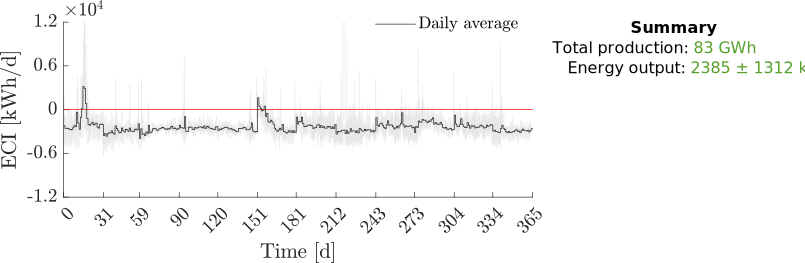
\includegraphics[width=0.8\textwidth]{figs/Simulation_ECI}}%
\end{center}

\vfill

\only<3>{
\boxInfo[0.85\textwidth]{ \centering
    The controller renders the WRRF energetically self-sufficient (on average)
}
}

\end{frame}
%------------------------------------------------------- 

%------------------------------------------------------- 
\begin{frame}[t]
\frametitle{Intro, control in (large-scale) cyber-physical systems}

\vfill
\begin{columns}
	\column[t]{0.6\textwidth}
	\begin{center}
		\vskip-1.5em
		\includegraphics[width=\textwidth]{figs/Game_Diagram}
	\end{center}

	\column[t]{0.4\textwidth}
	\vskip0.25em
	\textbf{\color{pastelGreen}Goal:} 
	\begin{itemize}
		\item [\color{pastelGreen}$\leadsto$] Optimal control in multi-agent settings
	\end{itemize}

	\vskip0.66em
	\onslide<2->{
	\textbf{\color{pastelRed}Challenges:}
	\begin{itemize}
		\item [\color{pastelRed}$\leadsto$] Large-scale network of subsystems
		\item [\color{pastelRed}$\leadsto$] Non-cooperative decision-making agents
		\item [\color{pastelRed}$\leadsto$] Subsystems are only partially observed
		\item [\color{pastelRed}$\leadsto$] Information exchange often asymmetric
	\end{itemize}
	}

	\vskip0.4cm
	\onslide<3->{
	\begin{center}
		\begin{tcolorbox}[boxrule=-5pt,width=20em,colback=white!95!black] \centering
			Feedback controllers (\textbf{control theory}) \\
			+ \\ 
			Equilibrium-seeking (\textbf{game theory})
		\end{tcolorbox}
	\end{center}
	}
\end{columns}

\vfill
\onslide<3->{
\begin{center}
	\begin{minipage}{0.75\textwidth}
		\begin{block}{} \centering
			We propose a systematic approach to \textbf{seeking feedback equilibrium strategies} in $N_P$-players non-cooperative dynamic games
		\end{block}
	\end{minipage}
\end{center}
}

\end{frame}

%------------------------------------------------------- 
\begin{frame}[t]
\frametitle{Intro, non-cooperative games and equilibrium-seeking}

\begin{block}{} \centering
	A non-cooperative game is defined as the tuple 
	\vskip-1.5em
	$$
	\mathcal{G} \coloneqq (\clP{\underbrace{\{ 1, \ldots, N_P \}}_{\text{set of players } \mathcal{P}}},~~ \textcolor{pastelGreen}{\underbrace{\{ L^1, \ldots, L^{N_P} \}}_{\text{objective functions}}},~~ \clPU{\underbrace{\{\mathcal{S}^1, \ldots, \mathcal{S}^{N_P}, \mathcal{S}^{\text{global}}\}}_{\text{admissible strategies}}})
	$$
\end{block}
\vskip1em

\begin{columns}
	\column[t]{0.52\textwidth}
	\onslide<2->{%
	\textcolor{monokaiOrange}{\textsc{Assumption:}} Players prefer best-response strategies
	$$
		BR^p(\clU{s^{-p}}) \coloneqq \argmin_{\clU{s^p} \in \clPU{\mathcal{S}^{p}}}\{~ \textcolor{pastelGreen}{L^{p}(\clU{s^p} \mid \clU{s^{-p}})} : (\clU{s^p}, \clU{s^{-p}})\in \clPU{\mathcal{S}^{\text{global}}} ~\} 
	$$
	}
	\vskip-2.5em
	\onslide<3->{%
	$$\Downarrow$$
	\only<-5>{\textcolor{monokaiOrange}{\textsc{Solution concept:}} generalized Nash equilibrium (GNE)}
	\only<6->{\textcolor{monokaiOrange}{\textsc{Solution concept (refined):}} variational GNE (vGNE)}
	$$
		\only<1-3>{\clU{(s^{1^{\star}}, \ldots, s^{N_P^{\star}})} \in BR^1(\clU{s^{-1^{\star}}}) \times \cdots \times BR^{N_P}(\clU{s^{-N_P^{\star}}})}
		\only<4-5>{\clU{s^{\star}} \in BR(\clU{s^{\star}})}
		\only<6->{\langle \textcolor{pastelGreen}{F(\clU{s^{\star}})}, \clU{s} - \clU{s^{\star}} \rangle \geq 0, \quad \clU{s} \in \clPU{\mathcal{S}_{\mathcal{G}}}}
	$$
	}
	\vskip-2.5em
	\only<-5>{\onslide<5->{%
	$$\Downarrow$$
	\textcolor{monokaiOrange}{\textsc{Problem statement:}} Fixed point problem 
	$$
	\text{Find } \clU{s^{\star}} \in \mathbb{R}^{N_s} \text{ such that } \clU{s^{\star}} \in BR(\clU{s^{\star}})
	$$
	}}
	\only<6->{\onslide<7->{%
	$$\Downarrow$$
	\textcolor{monokaiOrange}{\textsc{Problem statement:}} Monotone inclusion / VI problem$^{*}$
	$$
	\text{Find } \clU{s^{\star}} \in \mathbb{R}^{N_s} \text{ such that } 0 \in \textcolor{pastelGreen}{F(\clU{s^{\star}})} + \clPU{N_{\mathcal{S}_{\mathcal{G}}}(\clU{s^{\star}})}
	$$
	}}
	
	\column[t]{0.43\textwidth}
	\only<-5>{\onslide<5->{%
	\begin{center}
		\vskip-2em
		\begin{algorithm}[H]
			\caption{GNE-Seeking via BRD}
			% Initialize $s_{0} = (s_{0}^1,\ldots,s_{0}^{N_P})$ and $k = 0$\;
			\For{$k = 0, 1, 2, \ldots$}{ 
				\For{each player $\clP{p \in \mathcal{P}}$}{
					$\clU{s^p_{k+1}} \coloneqq (1-\clP{\eta})\clU{s^p_{k}} + \clP{\eta} BR^p(\clU{s^p_k}, \clU{s^{-p}_k})$\;
				}
			}
		\end{algorithm}
	\end{center}
	\vskip-1em
	\begin{columns}
	\column[t]{0.50\textwidth}
		\begin{itemize}
			\item[\color{glgGreen}$\checkmark$] Realistic routine
			\item[\color{glgGreen}$\checkmark$] Fully decentralised
		\end{itemize}
		
		\column[t]{0.54\textwidth}
		\begin{itemize}
			\item [\color{glgRed}$\times$] Scalability
			\item [\color{glgRed}$\times$] Robustness to errors
			\item [\color{glgRed}$\times$] Convergence guarantees
		\end{itemize}
	
	\end{columns}
	}}
	\only<6->{\onslide<7->{%
	\begin{center}
		\vskip-2em
		\begin{algorithm}[H]
			\caption{vGNE-Seeking via FB-Splitting}
			% Initialize $s_{0} = (s_{0}^1,\ldots,s_{0}^{N_P})$ and $k = 0$\;
			\For{$k = 0, 1, 2, \ldots$}{ 
				\For{each player $\clP{p \in \mathcal{P}}$}{
					$\clU{s^p_{+}} \coloneqq \clU{s^p_{k}} - \clP{\eta} \nabla \textcolor{pastelGreen}{L^p(\clU{s^p_k} \mid \clU{s^{-p}_k})}$\;
				}
				\For{coordinator}{
					$\clU{s_{k+1}} \coloneqq \mathrm{proj}_{\clPU{\mathcal{S}_{\mathcal{G}}}}(\clU{s_{+}})$\;
				}
			}
		\end{algorithm}
	\end{center}
	\vskip-1em
	\begin{columns}
	\column[t]{0.50\textwidth}
		\begin{itemize}
			\item[\color{glgGreen}$\checkmark$] Realistic routine
			\item[\color{glgGreen}$\checkmark$] (Often) scalable
			\item[\color{glgGreen}$\checkmark$] Convergence guarantees
		\end{itemize}
	
	\column[t]{0.54\textwidth}
		\begin{itemize}
			\item[\color{glgRed}$\times$] Semi-decentralised
			\item[\color{glgRed}$\times$] Robustness to errors
		\end{itemize}
	
	\end{columns}
	}}
\end{columns}

\only<6->{
\vfill\vskip1.2em
\textcolor{gray}{\footnotesize
	\hrule\vskip0.5em
	$^{*}$Assuming $F(s) = \big( \nabla L^p(s^p \mid s^{-p}) \big)_{p\in\mathcal{P}}$ is maximal monotone and $\mathcal{S}_{\mathcal{G}} = (\mathcal{S}^1 \times \cdots \times \mathcal{S}^{N_P}) \cap \mathcal{S}^{\text{global}}$ is closed convex
}
}

\end{frame}
	
%------------------------------------------------------- 
\begin{frame}[c]
\frametitle{GFNE, problem formulation for (stochastic) dynamic games}

\begin{center}
	\begin{minipage}{0.85\textwidth}

		\textcolor{monokaiOrange}{\sc (Stochastic) Dynamic games} \\[-2ex]
		\begin{block}{} \centering
			In \textit{(stationary) feedback Nash equilibrium} problems $\mathcal{G}_{\infty}^{\text{LQ}}$, strategies are feedback policies 
			$$
				\hspace*{-4em} \clU{s^p} \leadsto \qquad \clPU{K^p} : \clX{x_t} \mapsto \clU{u_t} \coloneqq \clPU{\Phi_{K}^p} * \clX{x_t} 
			$$
			computing \clU{actions ($u = (u^1, \ldots, u^{N_P})$)} to stabilize the \clX{state ($x$)} of the stochastic system
			$$
				\clX{x_{t+1}} = \clP{A} \clX{x_{t}} + \textstyle\sum_{p} \clP{B_u^p} \clU{u_t^p} + \clW{w_t} 
			$$
			while satisfying both \textbf{structural} (on $\clPU{K^p}$) and \textbf{operational} (on \{$\clX{x}$, $\clU{u}$\}) constraints
		\end{block}
	\end{minipage}
\end{center}

\end{frame}

%------------------------------------------------------- 
\begin{frame}[t]
\frametitle{GFNE, problem formulation and system level parametrisation}

\begin{center}
	\vskip-0.33em
	\begin{block}{}
		\only<1-2>{\vskip-1em
		$$	\hspace*{1em}
			BR^{p}(\clPU{K^{-p}}) :
			\left\{\begin{aligned}
				\underset{\clPU{K^p}}{\text{minimize}} \quad 
					& \mathrm{E}\left[\sum_{t=0}^{\infty} \Big( \| \clP{W_x^p} \clX{x_t} \|_2^2 + \| \clP{W_u^p} \clU{u_t^p} \|_2^2 \Big) \right] \\[0.5ex]
				\underset{\scriptsize\begin{matrix} \forall t \in \mathbb{N} \\ \forall \bar{p} \in \mathcal{P} \end{matrix}}{\text{subject to}} \quad
					& \clX{x_{t+1}}       = \clP{A} \clX{x_{t}} + \textstyle\sum_{\bar{p}} \clP{B_u^{\bar{p}}} \clU{u^{\bar{p}}_{t}} + \clW{w_t}, \quad \clX{x_0} = 0 & \textcolor{gray}{\footnotesize\text{[dynamics]}} \\[-4ex]
					& \clU{u^{\bar{p}}_t} = \clPU{\Phi_K^{\bar{p}}} * \clY{x_t}, & \textcolor{gray}{\footnotesize\text{[control policy]}}\\
					& \clPU{K^p} \in \{ \clPU{\text{Stability constraints}} \} \cap \{ \clPU{\text{Information constraints}} \}, & \textcolor{gray}{\footnotesize\text{[struct. constraints]}}  \\
					& \clP{G_x} \clX{x_t} + \clP{G_u^p} \clU{u_t} \preceq 1  & \textcolor{gray}{\footnotesize\text{[operat. constraints]}} 
			\end{aligned}\right.
		$$
		}%
		\only<3>{
		$$ \hspace*{-5em}
			BR^{p}_{\Phi}(\clPU{\bm \Phi_u^{-p}}) :
			\left\{\begin{aligned}
				\underset{\clPU{\Phi_u^p}}{\text{minimize}} \quad 
					& \sum_{n=0}^{\infty} \Big( \| \clP{W_x^p} \clPX{\Phi_{x,n}} \clP{B_w} \|_F^2 + \| \clP{W_u^p} \clPU{\Phi_{u,n}^p} \clP{B_w} \|_F^2 \Big) \\[0.5ex]
				\underset{\scriptsize\begin{matrix} \forall n \in \mathbb{N} \\ \forall \bar{p} \in \mathcal{P} \end{matrix}}{\text{subject to}} \quad
					& \clPU{\Phi_u^p}*\clPX{\Phi_x^{-1}} \in \{ \clPU{\text{Stability constraints}} \} \cap \{ \clPU{\text{Information constraints}} \}, \\[-4ex]
					& (\clP{G_x} \clPX{\Phi_x} + \clP{G_u^p} \clPU{\Phi_u})*\clW{w_n} \preceq 1 \\
			\end{aligned}\right.
		$$
		}%
		\only<4>{
		$$ \hspace*{-12em}
			BR^{p}_{\Phi}(\clPU{\bm \Phi_u^{-p}}) :
			\left\{\begin{aligned}
				\underset{\clPU{\Phi_u^p}}{\text{minimize}} \quad 
					& \sum_{n=0}^{\infty} \Big( \| \clP{W_x^p} \clPX{\Phi_{x,n}} \clP{B_w} \|_F^2 + \| \clP{W_u^p} \clPU{\Phi_{u,n}^p} \clP{B_w} \|_F^2 \Big) \\[0.5ex]
				\underset{\scriptsize\begin{matrix} \forall n \in \mathbb{N} \\ \forall \bar{p} \in \mathcal{P} \end{matrix}}{\text{subject to}} \quad
					& \clPX{\Phi_{x,n+1}} = \clP{A} \clPX{\Phi_{x,n}} + \textstyle\sum_{\bar{p}} \clP{B_u^{\bar{p}}} \clPU{\Phi_{u,n}^{\bar{p}}}, \quad \clPX{\Phi_{x,1}} = I_{N_x}\\[-4ex]
					& \clPU{\Phi_u^p}*\clPX{\Phi_x^{-1}} \in \{ \clPU{\text{Information constraints}} \}, \\
					& (\clP{G_x} \clPX{\Phi_x} + \clP{G_u^p} \clPU{\Phi_u})*\clW{w_n} \preceq 1
			\end{aligned}\right.
		$$
		}%
		\only<5>{\vskip-1em
		$$ \hspace*{1em}
			BR^{p}_{\Phi}(\clPU{\bm \Phi_u^{-p}}) :
			\left\{\begin{aligned}
				\underset{\clPU{\Phi_u^p}}{\text{minimize}} \quad 
					& \sum_{n=0}^{N-1} \Big( \| \clP{W_x^p} \clPX{\Phi_{x,n}} \clP{B_w} \|_F^2 + \| \clP{W_u^p} \clPU{\Phi_{u,n}^p} \clP{B_w} \|_F^2 \Big) +  \| \clP{W_f} \clPX{\Phi_{x,N}} \clP{B_w} \|_F^2 \\[0.5ex]
				\underset{\scriptsize\begin{matrix} \forall n \in \mathbb{N} \\ \forall \bar{p} \in \mathcal{P} \end{matrix}}{\text{subject to}} \quad
					& \clPX{\Phi_{x,n+1}} = \clP{A} \clPX{\Phi_{x,n}} + \textstyle\sum_{\bar{p}} \clP{B_u^{\bar{p}}} \clPU{\Phi_{u,n}^{\bar{p}}}, \quad \clPX{\Phi_{x,1}} = I_{N_x}\\[-4ex]
					& \mathtt{Sp}(\clPX{\Phi_{x,n}}) = \mathtt{Sp}(\clP{S_n}), \quad \mathtt{Sp}(\clPU{\Phi_{u,n}^p}) = \mathtt{Sp}(\clP{B_u^{p^\tran}}\clP{S_n}), &\hspace*{-5em} \text{w/ } \clP{S_n} = \clP{A}^{\min(0, \lfloor n-\clP{d_a} / \clP{d_c} \rfloor)}, \\
					& (\clP{G_x} \clPX{\Phi_x} + \clP{G_u^p} \clPU{\Phi_u})*\clW{w_n} \preceq 1
			\end{aligned}\right.
		$$
		}%
		\only<6->{\vskip-1em
		$$ \hspace*{1em}
			BR^{p}_{\Phi}(\clPU{\bm \Phi_u^{-p}}) :
			\left\{\begin{aligned}
				\underset{\clPU{\Phi_u^p}}{\text{minimize}} \quad 
					& \sum_{n=0}^{N-1} \Big( \| \clP{W_x^p} \clPX{\Phi_{x,n}} \clP{B_w} \|_F^2 + \| \clP{W_u^p} \clPU{\Phi_{u,n}^p} \clP{B_w} \|_F^2 \Big) +  \| \clP{W_f} \clPX{\Phi_{x,N}} \clP{B_w} \|_F^2 \\[0.5ex]
				\underset{\scriptsize\begin{matrix} \forall n \in \mathbb{N} \\ \forall \bar{p} \in \mathcal{P} \end{matrix}}{\text{subject to}} \quad
					& \clPX{\Phi_{x,n+1}} = \clP{A} \clPX{\Phi_{x,n}} + \textstyle\sum_{\bar{p}} \clP{B_u^{\bar{p}}} \clPU{\Phi_{u,n}^{\bar{p}}}, \quad \clPX{\Phi_{x,1}} = I_{N_x}\\[-4ex]
					& \mathtt{Sp}(\clPX{\Phi_{x,n}}) = \mathtt{Sp}(\clP{S_n}), \quad \mathtt{Sp}(\clPU{\Phi_{u,n}^p}) = \mathtt{Sp}(\clP{B_u^{p^\tran}}\clP{S_n}), &\hspace*{-5em} \text{w/ } \clP{S_n} = \clP{A}^{\min(0, \lfloor n-\clP{d_a} / \clP{d_c} \rfloor)}, \\
					& (\clP{G_{x,i}} \clPX{\Phi_x}\clP{B_w} + \clP{G_{u,i}^p} \clPU{\Phi_u} \clP{B_w})^{\tran}  \preceq_{K_2} 1/Q(\clP{\rho}),  &\hspace*{-5em} (\forall i) 
			\end{aligned}\right.
		$$
		}%
	\end{block}
\end{center}

\only<1-2>{
\begin{flushright}
	\vskip-12.5em
	\textcolor{gray}{\footnotesize
		$w$ is a AWGN process, that is,\\[-0.5ex] 
		$\mathbb{E}w_t = 0$ and $\mathbb{E}(w_t w_{t-\tau}^{\tran}) = \delta_{\tau}B_w B_w^{\tran}$
	}
	\vskip10em
\end{flushright}
}

\only<1>{
	\vfill
	\begin{columns}
		\column[c]{0.5\textwidth}
		\textsc{\textcolor{glgRed}{Problem:}}
		\begin{center}
			\begin{tcolorbox}[boxrule=-5pt,width=24em,colback=white!90!glgRed] \centering
				The fixed-points of $BR(\cdot)$ cannot be searched through monotone inclusion problems
				$$ 
				\Downarrow
				$$
				!! No systematic method to compute GFNEs !!
			\end{tcolorbox}
		\end{center}

		\column[c]{0.5\textwidth}
		\textsc{\textcolor{glgGreen}{Solution:}}
		\begin{center}
			\begin{tcolorbox}[boxrule=-5pt,width=24em,colback=white!90!glgGreen] \centering
				A parametrisation of $K^p$ to design an alternative but equivalent $BR(\cdot)$ mapping
				$$ 
				\Downarrow
				$$
				\textbf{System level synthesis (SLS)}
			\end{tcolorbox}
		\end{center}
	\end{columns}
	\vfill
}
\only<2-6>{
	\vskip0.33em
	\begin{columns}\small
		\column[t]{0.5\textwidth}%
		\textcolor{monokaiOrange}{\textsc{Step 1) System-level responses (frequency domain)}}
		$$\begin{aligned}
			\clX{\bm x  } &= \big(\clP{zI{-}A} + \textstyle\sum_p \clP{B_u^p} \clPU{\bm K^p}\big)^{-1} \clW{\bm w}  			  &= \clPX{\bm \Phi_x}   \clW{\bm w} \\[-0.5ex]
			\clU{\bm u^p} &= \clPU{\bm K^p} \big(\clP{zI{-}A} + \textstyle\sum_p \clP{B_u^p} \clPU{\bm K^p}\big)^{-1} \clW{\bm w} &= \clPU{\bm \Phi_u^p} \clW{\bm w} \\[-0.5ex]
			\clPU{\bm \Phi_K^p} &= \clPU{\bm \Phi_u^p} \clPX{\bm \Phi_x^{-1}}
		\end{aligned}$$

		\onslide<4->{%
		\textcolor{monokaiOrange}{\textsc{Step 2) System-level parametrisation (time domain)}}
		\begin{center}
			Stability $\iff$ 
			$\begin{aligned}
				\clPX{\Phi_{x,n+1}} &= \clP{A}\clPX{\Phi_{x,n}} + \textstyle\sum_{p} \clP{B_u^p} \clPU{\Phi_{u,n}^p}\\[-1ex]
				\clPX{\Phi_{x,1}} &= I_{N_x}
			\end{aligned}$
		\end{center}
		}%

		\column[t]{0.5\textwidth}
		\onslide<5->{%
		\textcolor{monokaiOrange}{\textsc{Step 3) System-level constraints}}\\[-0.75ex]
		\textcolor{gray}{\footnotesize(leading to a finite-horizon optimization problem)}
		\begin{multline*}
			\clPX{\Phi_x}, \clPU{\Phi_u^p} \in \big\{ \text{FIR w/ } N \text{ factors} \big\} \\
				\cap \text{\{ Information as sparsity constraints \}}
		\end{multline*}
		}%

		\onslide<6->{%
		\textcolor{monokaiOrange}{\textsc{Step 4) Expectation and chance constraints}}\\[-0.75ex]
		\textcolor{gray}{\footnotesize(leading to second-order conic constraints)}
		$$
			\mathbf{prob}\big[(\text{\clPX{st}\clPU{uff}})*\clW{w_n} \leq 1\big] \geq \clP{\rho} \iff \| \clP{B_w^{\tran}}(\text{\clPX{st}\clPU{uff}})^{\tran} \|_{\ell_2} \leq 1/Q(\clP{\rho})
		$$
		}

	\end{columns}
}

\only<7->{
\begin{columns}
	\column[t]{0.5\textwidth}
	\begin{center}
		\begin{tcolorbox}[boxrule=-5pt,width=24em,colback=white!90!glgGreen] \centering
			$\clPU{K^{\star}}$ is a vGFNE of $\mathcal{G}_{\infty}^{\text{LQ}}$ \textcolor{gray}{[dynamic game]}
			$$\Updownarrow$$
			$\clPU{\Phi_u^{\star}}$ is a vGNE of $\mathcal{G}_{\Phi}^{\text{LQ}}$ \textcolor{gray}{[static game]}
		\end{tcolorbox}
	\end{center}

	\column[t]{0.46\textwidth}
	\vskip-1.5em
	\begin{algorithm}[H]
		\caption{vGFNE-Seeking via FB-Splitting}
		% Initialize $\Phi_{u,0} = (\Phi_{u,0}^1, \ldots, \Phi_{u,0}^{N_P})$ and $k = 0$\;
		\For{$k = 0, 1, 2, \ldots$}{ 
			\For{each player $\clP{p \in \mathcal{P}}$}{
				$\clPU{\bm{K}_k^p} \coloneqq \clPU{\bm{\Phi_{u,k}}^p} \clPX{\bm{\Phi_{x,k}}^{-1}}$\;
				$\clPU{\bm{\Phi}_{u,+}^p} \coloneqq \clPU{\bm{\Phi}_{u,k}^p} - \clP{\eta} \nabla \textcolor{pastelGreen}{L_{\Phi}^p(\clPU{\bm{\Phi}_{u,k}^p} \mid \clPU{\bm{\Phi}_{u,k}^{-p}})}$\;
			}
			\For{coordinator}{
				$\clPU{\bm{\Phi}_{u,k+1}} \coloneqq \mathrm{proj}_{\clPU{\mathcal{U}_{\bm{\Phi},\mathcal{G}}}}(\clPU{\bm{\Phi}_{u,+}})$\;
			}
		}
	\end{algorithm}
	
\end{columns}
}
		
\end{frame}

%------------------------------------------------------- 
\begin{frame}[c]
\frametitle{GFNE, partially-observed dynamic games}

\begin{center}
	\begin{tcolorbox}[boxrule=-5pt,width=0.85\textwidth,colback=white!95!monokaiBG] \centering
		What about \textbf{partially-observed} (i.e., output-feedback) Nash equilibrium problems?
		$$
		\left\{ 
			\begin{aligned}
				\clX{x_{t+1}} &= \clP{A} \clX{x_{t}} + \textstyle\sum_{p} \clP{B_u^p} \clU{u_t^p} + \clW{w_t} \\ 
				\clY{y_t}     &= \clP{C} \clX{x_{t}} + \clW{v_t} \\ 
				\clU{u_t^p}     &= \clPU{K^p} * \clY{y_t}
			\end{aligned}
		\right.
		\qquad \Rightarrow\qquad
		\left\{ 
			\begin{aligned}
				\clX{\bm x}    &= \clPX{\bm \Phi_{xx}} \clW{\bm w} + \clPX{\bm \Phi_{xy}} \clW{\bm v} \\
				\clU{\bm u^p}  &= \clPU{\bm \Phi_{ux}^p} \clW{\bm w} + \clPU{\bm \Phi_{uy}^p} \clW{\bm v} \\
				\clPU{\bm K^p} &= \clPU{\bm \Phi_{uy}^p} - \clPU{\bm \Phi_{ux}^p}\clPX{\bm \Phi_{xy}^{-1}}\clPX{\bm \Phi_{xy}}
			\end{aligned}
		\right.
		$$
	\end{tcolorbox}

	\vskip2em 

	\begin{columns} 
		\column{0.3\textwidth} \centering
		\includegraphics[width=0.8\textwidth]{figs/yes}
		
		\column{0.6\textwidth} \large
		\begin{itemize}
			\item [$\leadsto$]  Similar procedure (with much more involved formulas) so I will spare you the long details!
		\end{itemize}
	\end{columns}
\end{center}

\end{frame}

%------------------------------------------------------- 
\begin{frame}[t]
\frametitle{Example, power-grid with capacity constraints}

\begin{columns}
	\column[t]{0.42\textwidth}
	\begin{center}
		\vskip-1.2em
		
\includegraphics[width=\textwidth]{figs/PowerGrid.pdf}
	\end{center}

	\column[t]{0.50\textwidth}
	\textsc{\textcolor{monokaiOrange}{Continuous-time dynamics (each node):}}
	$$
		\clP{m^p} \clX{\ddot{\theta}^p} + \clP{d^p} \clX{\dot{\theta}^p} = -\textstyle\sum_{\tilde{p}\in\mathcal{P}} \clP{\kappa^{p,\tilde{p}}}(\clX{\theta^p} - \clX{\theta^{\tilde{p}}}) + \clU{u^p} + \clW{\delta_x^p}
	$$

	\textsc{\textcolor{monokaiOrange}{Link capacity constraint (each node):}}
	$$
	-5 \leq  \clP{\kappa^{p,\tilde{p}}}(\clX{\theta^p} - \clX{\theta^{\tilde{p}}}) \leq 5, \quad \forall t \in \mathbb{N},~ \tilde{p} \in \mathcal{P}
	$$
\end{columns}

\separatorLine{1.5em}{0.5em}

\begin{columns}
	\column[t]{0.45\textwidth}
	\begin{center}
		\includegraphics[width=\textwidth]{figs/PGrid_Convergence}
	\end{center}
	\vskip-1em
	\begin{block}{} \centering
		Convergence to vGFNE \textcolor{gray}{(albeit slow)} while ensuring stability and constraint satisfaction
	\end{block}

	\column[t]{0.50\textwidth}
	\begin{center}
		\includegraphics[width=\textwidth]{figs/PGrid_Simulation_Optimized}
	\end{center}

\end{columns}

\end{frame}

% THANK YOU PAGE --------------------------------------------------------------
{\1
\begin{frame}[c,plain,noframenumbering]  
	\begin{center}
		\vfill
		\vskip5em

		% \textcolor{monokaiOrange}{\bf I am always looking for opportunities to collaborate-- so hit me up!}
		\vskip4em 

		\begin{minipage}{0.2\textwidth} \centering
			\includegraphics[scale=0.2]{figs/website.png}\\
			\textcolor{monokaiOrange}{\tt [tiominho.github.io]}
		\end{minipage}
		\hspace*{4em}
		\begin{minipage}{0.25\textwidth} \centering
			\includegraphics[scale=0.8]{figs/koira}\\
			{\bf \Huge \color{monokaiBG!25!white} Thank you!}\\
			{\Large \color{monokaiOrange} \textbf{Questions?}}\\
		\end{minipage}

		\vfill
		\vskip4em
		{\bfseries \color{monokaiOrange} \insertshorttitle}\\
		{\color{monokaiOrange}May 26, 2025}
	\end{center}
\end{frame}
}

%-------------------------------------------------------
\end{document}